\documentclass[tikz,border=3pt]{standalone}
\usepackage[utf8]{inputenc}
\usepackage[T1]{fontenc}
\usepackage{lmodern}
\renewcommand{\familydefault}{\sfdefault}
\usepackage{sansmath}\sansmath
\usepackage{pgfplots}\pgfplotsset{compat=1.18,/pgf/number format/use comma,/pgf/number format/1000 sep={.}}
\usetikzlibrary{arrows.meta,calc,positioning,decorations.pathmorphing,patterns}
% paleta del sitio
\definecolor{nar}{HTML}{E8680C}\definecolor{narc}{HTML}{FFB35C}\definecolor{hielo}{HTML}{FFF3E8}
\definecolor{tinta}{HTML}{1D1D1F}\definecolor{gris}{HTML}{6E6E73}\definecolor{lila}{HTML}{7C5CF0}
\definecolor{azul}{HTML}{2F6FD6}\definecolor{menta}{HTML}{17A673}\definecolor{coral}{HTML}{E8342A}
\begin{document}
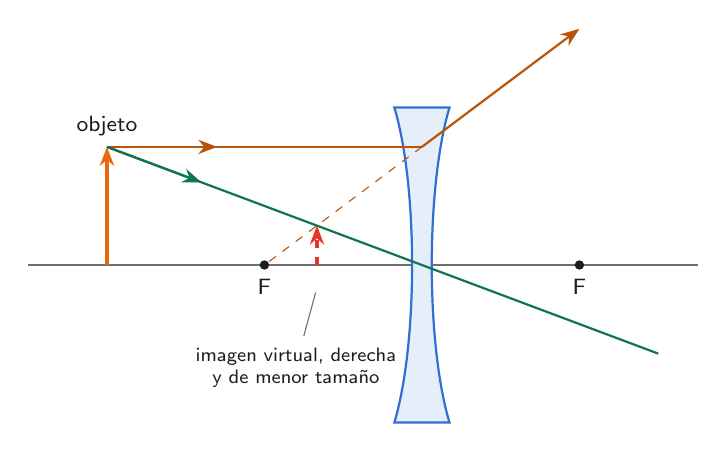
\begin{tikzpicture}[font=\footnotesize,>={Stealth[length=2.4mm]}]
\draw[gris] (-5,0) -- (3.5,0);
\draw[thick,azul,fill=azul!12] (-0.35,2) -- (0.35,2) .. controls (0.05,1) and (0.05,-1) .. (0.35,-2) -- (-0.35,-2) .. controls (-0.05,-1) and (-0.05,1) .. (-0.35,2) -- cycle;
\foreach \x/\t in {-2/F,2/F} {\fill[tinta] (\x,0) circle (0.06); \node[below,text=tinta] at (\x,-0.05) {\t};}
\draw[->,line width=1.6pt,nar] (-4,0) -- (-4,1.5) node[above,text=tinta] {objeto};
\draw[nar!80!black,thick] (-4,1.5) -- (0,1.5); \draw[->,nar!80!black,thick] (-4,1.5) -- (-2.6,1.5);
\draw[->,nar!80!black,thick] (0,1.5) -- (2,3.0);
\draw[nar!80!black,thin,dashed] (0,1.5) -- (-2,0);
\draw[menta!70!black,thick] (-4,1.5) -- (3,-1.125); \draw[->,menta!70!black,thick] (-4,1.5) -- (-2.8,1.05);
\draw[->,line width=1.6pt,coral,dashed] (-1.333,0) -- (-1.333,0.5);
\node[text=tinta,align=center,font=\scriptsize] at (-1.6,-1.3) {imagen virtual, derecha\\y de menor tamaño};
\draw[gris,thin] (-1.35,-0.35) -- (-1.5,-0.9);
\end{tikzpicture}
\end{document}
